\documentclass[a4paper,11pt,oneside]{book}
\usepackage[pdftex,bookmarks=true,bookmarksnumbered=true]{hyperref}
\usepackage{xcolor}
\usepackage{textcomp} % Copyright sign
\usepackage[utf8]{inputenc}
\usepackage{xspace}

\usepackage{graphicx}
\graphicspath{{images/}}

\usepackage[
    backend=biber
]{biblatex}
\addbibresource{literature.bib}

\hypersetup
{
  bookmarksnumbered = true,
  pdfauthor = Johannes Natter
  pdftitle = Visual Software Editor - vised,
  pdfsubject = ,
  pdfkeywords = ,
  pdfcreator = ,
  pdfproducer = ,
  colorlinks = true,
  linkcolor = black,
  citecolor = black,
  filecolor = black,
  urlcolor = black
}
\usepackage{epstopdf}
\usepackage{pdfsync}

% Commands
\newcommand{\todo}[1]{\textbf{\textcolor{red}{TODO: #1}}\\}
\newcommand{\vised}{\emph{vised}\xspace}

\begin{document}

  \title{\textbf{Visual Software Editor \\ \vised}} 
  \author{Johannes Natter}
  \date{\today \\ \vspace{5cm} 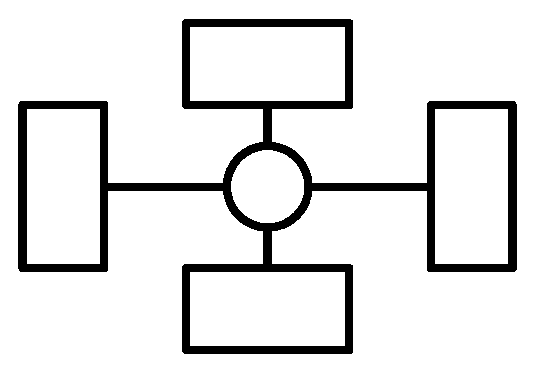
\includegraphics[width=100 pt]{../_common/logo}}

  % Intro
  \frontmatter
  \maketitle
  
\chapter*{}

\vspace{5cm}
\begin{center}
    \copyright\ Copyright\ \the\year\ Johannes Natter
\end{center}
\vspace{0.7cm}
This document is published under the terms of the \emph{GNU General Public License Version 2} (GNU GPLv2).
See \url{http://www.gnu.org/licenses/gpl-2.0.html} for more information.


  \tableofcontents
  % -----------------------------------------------------------------------------
% -----------------------------------------------------------------------------
% --                                                                         --
% --  This file is part of the Visual Software Editor project                --
% --  https://github.com/Naegolus/vised                                      --
% --                                                                         --
% --  Author(s):                                                             --
% --      - Helmut, redrocket@gmx.at                                         --
% --                                                                         --
% -----------------------------------------------------------------------------
% --                                                                         --
% --  Copyright (C) 2015 Authors                                             --
% --                                                                         --
% --  This program is free software: you can redistribute it and/or modify   --
% --  it under the terms of the GNU General Public License as published by   --
% --  the Free Software Foundation, either version 3 of the License, or      --
% --  (at your option) any later version.                                    --
% --                                                                         --
% --  This program is distributed in the hope that it will be useful,        --
% --  but WITHOUT ANY WARRANTY; without even the implied warranty of         --
% --  MERCHANTABILITY or FITNESS FOR A PARTICULAR PURPOSE. See the           --
% --  GNU General Public License for more details.                           --
% --                                                                         --
% --  You should have received a copy of the GNU General Public License      --
% --  along with this program. If not, see <http://www.gnu.org/licenses/>.   --
% --                                                                         --
% -----------------------------------------------------------------------------
% -----------------------------------------------------------------------------

\chapter{Abstract}

Lorem ipsum dolor sit amet, consectetur adipisicing elit, sed do eiusmod tempor incididunt ut
labore et dolore magna aliqua. Ut enim ad minim veniam, quis nostrud exercitation ullamco
laboris nisi ut aliquip ex ea commodo consequat. Duis aute irure dolor in reprehenderit in
voluptate velit esse cillum dolore eu fugiat nulla pariatur. Excepteur sint occaecat cupidatat
non proident, sunt in culpa qui officia deserunt mollit anim id est laborum \cite{freeman2004}.

Lorem ipsum dolor sit amet, consectetur adipisicing elit, sed do eiusmod tempor incididunt ut
labore et dolore magna aliqua. Ut enim ad minim veniam, quis nostrud exercitation ullamco
laboris nisi ut aliquip ex ea commodo consequat. Duis aute irure dolor in reprehenderit in
voluptate velit esse cillum dolore eu fugiat nulla pariatur. Excepteur sint occaecat cupidatat
non proident, sunt in culpa qui officia deserunt mollit anim id est laborum \cite{freeman2004}.

Lorem ipsum dolor sit amet, consectetur adipisicing elit, sed do eiusmod tempor incididunt ut
labore et dolore magna aliqua. Ut enim ad minim veniam, quis nostrud exercitation ullamco
laboris nisi ut aliquip ex ea commodo consequat. Duis aute irure dolor in reprehenderit in
voluptate velit esse cillum dolore eu fugiat nulla pariatur. Excepteur sint occaecat cupidatat
non proident, sunt in culpa qui officia deserunt mollit anim id est laborum \cite{freeman2004}.



  % Document
  \mainmatter
  
\chapter{Introduction}

\section{Editing Software then}

\section{Editing Software now}

\section{Target of this work}

\todo{This document should specify the first version of \vised}

\section{Notation}


  
\chapter{Existing systems}

\todo{positive}

\section{Many ways}

\todo{Full IDE, minimalistic, everthing in between}

\section{Microsoft Visual Studio}

\section{Eclipse}

\section{Enterprise Architect}

\section{Emacs}

\section{vim}

\section{...}


  % -----------------------------------------------------------------------------
% -----------------------------------------------------------------------------
% --                                                                         --
% --  This file is part of the Visual Software Editor project                --
% --  https://github.com/Naegolus/vised                                      --
% --                                                                         --
% --  Author(s):                                                             --
% --      - Helmut, redrocket@gmx.at                                         --
% --                                                                         --
% -----------------------------------------------------------------------------
% --                                                                         --
% --  Copyright (C) 2015 Authors                                             --
% --                                                                         --
% --  This program is free software: you can redistribute it and/or modify   --
% --  it under the terms of the GNU General Public License as published by   --
% --  the Free Software Foundation, either version 3 of the License, or      --
% --  (at your option) any later version.                                    --
% --                                                                         --
% --  This program is distributed in the hope that it will be useful,        --
% --  but WITHOUT ANY WARRANTY; without even the implied warranty of         --
% --  MERCHANTABILITY or FITNESS FOR A PARTICULAR PURPOSE. See the           --
% --  GNU General Public License for more details.                           --
% --                                                                         --
% --  You should have received a copy of the GNU General Public License      --
% --  along with this program. If not, see <http://www.gnu.org/licenses/>.   --
% --                                                                         --
% -----------------------------------------------------------------------------
% -----------------------------------------------------------------------------

\chapter{Introducing \vised}

\todo{Possible functions of the Software will be introduced}

\section{Goal}

\todo{What should \vised make better?}

\section{Interface}

\todo{Function: Required}

\section{Parsing programming language}

\todo{Function: Required}

\section{Automatic graph}

\todo{Function: Required}

\section{Undo/Redo}

\todo{Function: Required}

\section{Concurrent editing with external programs}

\todo{Function: Required}

\section{Views}

\todo{Function: Required}

\section{GIT}

\todo{Function: Required}

\section{Using external programs}

\todo{Function: Optional}

\section{Supporting design pattern}

\todo{Function: Optional}

\subsection{Structural/Behavioral/Concurrent pattern}

\section{Supported languages}

\todo{Function: C++ only}

\section{Server/Client}

\todo{Function: Obsolete}

\section{Graphics backend}

\todo{Function: Obsolete}

\section{System documentation}

\todo{Function: Obsolete}

\section{Minimap}

\todo{Function: Obsolete}

\section{Software debugging}

\todo{Function: Obsolete}

\section{Hardware Software codesign}

\todo{Function: Obsolete}


  
\chapter{Software architecture}

\todo{Architecture of core functionality}


  % -----------------------------------------------------------------------------
% -----------------------------------------------------------------------------
% --                                                                         --
% --  This file is part of the Visual Software Editor project                --
% --  https://github.com/Naegolus/vised                                      --
% --                                                                         --
% --  Author(s):                                                             --
% --      - Helmut, redrocket@gmx.at                                         --
% --                                                                         --
% -----------------------------------------------------------------------------
% --                                                                         --
% --  Copyright (C) 2015 Authors                                             --
% --                                                                         --
% --  This program is free software: you can redistribute it and/or modify   --
% --  it under the terms of the GNU General Public License as published by   --
% --  the Free Software Foundation, either version 3 of the License, or      --
% --  (at your option) any later version.                                    --
% --                                                                         --
% --  This program is distributed in the hope that it will be useful,        --
% --  but WITHOUT ANY WARRANTY; without even the implied warranty of         --
% --  MERCHANTABILITY or FITNESS FOR A PARTICULAR PURPOSE. See the           --
% --  GNU General Public License for more details.                           --
% --                                                                         --
% --  You should have received a copy of the GNU General Public License      --
% --  along with this program. If not, see <http://www.gnu.org/licenses/>.   --
% --                                                                         --
% -----------------------------------------------------------------------------
% -----------------------------------------------------------------------------

\chapter{Conclusion}


  
\chapter{Lorem ipsum}

Lorem ipsum dolor sit amet, consectetur adipisicing elit, sed do eiusmod tempor incididunt ut
labore et dolore magna aliqua. Ut enim ad minim veniam, quis nostrud exercitation ullamco
laboris nisi ut aliquip ex ea commodo consequat. Duis aute irure dolor in reprehenderit in
voluptate velit esse cillum dolore eu fugiat nulla pariatur. Excepteur sint occaecat cupidatat
non proident, sunt in culpa qui officia deserunt mollit anim id est laborum \cite{freeman2004}.

\section{Lorem}

Lorem ipsum dolor sit amet, consectetur adipisicing elit, sed do eiusmod tempor incididunt ut
labore et dolore magna aliqua. Ut enim ad minim veniam, quis nostrud exercitation ullamco
laboris nisi ut aliquip ex ea commodo consequat. Duis aute irure dolor in reprehenderit in
voluptate velit esse cillum dolore eu fugiat nulla pariatur. Excepteur sint occaecat cupidatat
non proident, sunt in culpa qui officia deserunt mollit anim id est laborum \cite{freeman2004}.

\subsection{ipsum}

Lorem ipsum dolor sit amet, consectetur adipisicing elit, sed do eiusmod tempor incididunt ut
labore et dolore magna aliqua. Ut enim ad minim veniam, quis nostrud exercitation ullamco
laboris nisi ut aliquip ex ea commodo consequat. Duis aute irure dolor in reprehenderit in
voluptate velit esse cillum dolore eu fugiat nulla pariatur. Excepteur sint occaecat cupidatat
non proident, sunt in culpa qui officia deserunt mollit anim id est laborum \cite{freeman2004}.

Lorem ipsum dolor sit amet, consectetur adipisicing elit, sed do eiusmod tempor incididunt ut
labore et dolore magna aliqua. Ut enim ad minim veniam, quis nostrud exercitation ullamco
laboris nisi ut aliquip ex ea commodo consequat. Duis aute irure dolor in reprehenderit in
voluptate velit esse cillum dolore eu fugiat nulla pariatur. Excepteur sint occaecat cupidatat
non proident, sunt in culpa qui officia deserunt mollit anim id est laborum \cite{freeman2004}.

\section{dolor}

Lorem ipsum dolor sit amet, consectetur adipisicing elit, sed do eiusmod tempor incididunt ut
labore et dolore magna aliqua. Ut enim ad minim veniam, quis nostrud exercitation ullamco
laboris nisi ut aliquip ex ea commodo consequat. Duis aute irure dolor in reprehenderit in
voluptate velit esse cillum dolore eu fugiat nulla pariatur. Excepteur sint occaecat cupidatat
non proident, sunt in culpa qui officia deserunt mollit anim id est laborum \cite{freeman2004}.

Lorem ipsum dolor sit amet, consectetur adipisicing elit, sed do eiusmod tempor incididunt ut
labore et dolore magna aliqua. Ut enim ad minim veniam, quis nostrud exercitation ullamco
laboris nisi ut aliquip ex ea commodo consequat. Duis aute irure dolor in reprehenderit in
voluptate velit esse cillum dolore eu fugiat nulla pariatur. Excepteur sint occaecat cupidatat
non proident, sunt in culpa qui officia deserunt mollit anim id est laborum \cite{freeman2004}.

Lorem ipsum dolor sit amet, consectetur adipisicing elit, sed do eiusmod tempor incididunt ut
labore et dolore magna aliqua. Ut enim ad minim veniam, quis nostrud exercitation ullamco
laboris nisi ut aliquip ex ea commodo consequat. Duis aute irure dolor in reprehenderit in
voluptate velit esse cillum dolore eu fugiat nulla pariatur. Excepteur sint occaecat cupidatat
non proident, sunt in culpa qui officia deserunt mollit anim id est laborum \cite{freeman2004}.

Lorem ipsum dolor sit amet, consectetur adipisicing elit, sed do eiusmod tempor incididunt ut
labore et dolore magna aliqua. Ut enim ad minim veniam, quis nostrud exercitation ullamco
laboris nisi ut aliquip ex ea commodo consequat. Duis aute irure dolor in reprehenderit in
voluptate velit esse cillum dolore eu fugiat nulla pariatur. Excepteur sint occaecat cupidatat
non proident, sunt in culpa qui officia deserunt mollit anim id est laborum \cite{freeman2004}.



  \clearpage

  % Apendix
  \backmatter
  \IfFileExists{./todos.tex}{\include{todos}}{}

  % References
  \printbibliography

\end{document}

